%%%%%%%%%%%%%%%%%%%%%%%%%%%%%%%%%%%%%%%%%%%%%%%%%%%%%%%%%%%%%%%
%
% Welcome to Overleaf --- just edit your LaTeX on the left,
% and we'll compile it for you on the right. If you open the
% 'Share' menu, you can invite other users to edit at the same
% time. See www.overleaf.com/learn for more info. Enjoy!
%
%%%%%%%%%%%%%%%%%%%%%%%%%%%%%%%%%%%%%%%%%%%%%%%%%%%%%%%%%%%%%%%




\documentclass{report}
\usepackage{subfigure}
% \usepackage[albanian]{babel}
\usepackage{listings}
\usepackage{color}
\usepackage{graphicx}
\usepackage{pgfplots}
\usepackage{booktabs}
\usepackage{pgfplots}
\usepackage{pdfpages}
\pgfplotsset{compat=1.17}
\usepackage{hyperref}
\graphicspath{ {./images/} }


\usepackage{amsmath}
\usepackage{amsfonts}
\usepackage{amssymb}
\usepackage{amscd}
\usepackage{amsthm}

\definecolor{dkgreen}{rgb}{0,0.6,0}
\definecolor{gray}{rgb}{0.5,0.5,0.5}
\definecolor{mauve}{rgb}{0.58,0,0.82}

\lstset{frame=tb,
  language=C++,
  aboveskip=1mm,
  belowskip=1mm,
  showstringspaces=false,
  columns=flexible,
  basicstyle={\small\ttfamily},
  numbers=none,
  numberstyle=\tiny\color{gray},
  keywordstyle=\color{blue},
  commentstyle=\color{dkgreen},
  stringstyle=\color{mauve},
  numbers=left, % Add line numbering
  breaklines=true,
  breakatwhitespace=true,
  tabsize=1
}
\begin{document}

\renewcommand\bibname{Referencat}
\renewcommand{\chaptername}{Kapitulli}
\renewcommand{\contentsname}{Përmbajtja}
\renewcommand\appendixname{Apendiks}
\renewcommand{\figurename}{Figura}
\renewcommand{\tablename}{Tabela}

\newpage
\includepdf[pages={1}]{coverPage.pdf}
\renewcommand{\abstractname}{Deklaratë e autorësisë}
\begin{abstract}
Unë, Drilon Aliu, deklaroj me vetëdije dhe ndërgjegje të plotë që ky punim është rezultat i punës sime të pavarur dhe jam plotësisht i vetëdijshëm që plagjiarizëm konsiderohet kopjimi i punës së bërë nga të tjerët dhe paraqitja e saj si punë e imja. Në çdo rast të vetëm në këtë punim mbështetja e tërthortë apo citimi i drejtpërdrejtë në punën e autorëve të tjerë është e deklaruar si e tillë. Unë jam plotësisht i vetëdijshëm që plagjiarizmi rezulton automatikisht me notë negative dhe do të pasojnë masa disiplinore që mund të shpijnë deri te marrja e së drejtës për të qenë student/e në Universitetin e Prishtinës.\\
\end{abstract}



\renewcommand{\abstractname}{Abstrakt}
\begin{abstract}
Ky punim diplome shtjellon aplikimin e programimit paralel për të gjeneruar fraktalet. Fraktalet, për shkak të natyrës së tyre rekursive, paraqesin sfidë kompjutimi për iterime të larta, duke i bërë ato kandidatë idealë për përpunim paralel. Duke përdorur platformën CUDA me grupet kooperative, llogaritjet përshpejtohen dukshëm në krahasim me metodat tradicionale sekuenciale. Libraria OpenGL është përdorur për të vizualizuar fraktalet, dhe interoperabiliteti CUDA-OpenGL është shfrytëzuar me qëllimin që llogaritjet e shpejtuara në GPU të shfaqen direkt në OpenGL pa nevojën e transferimit të të dhënave në CPU.\\

\noindent \textbf{\textit{Fjalët Kyqe:}} \textit{fraktal, paralel, sekuencial, CUDA, OpenGL, iterim, rekursion, graf, kernel, memorie.}
\end{abstract}



\newpage
\renewcommand{\abstractname}{Abstract}
\begin{abstract}
This thesis elaborates on the application of parallel programming to generate fractals. Fractals, due to their recursive nature, present a computational challenge for higher iterations, making them ideal candidates for parallel processing. Using NVIDIA's CUDA platform with cooperative groups, calculations are significantly accelerated compared to traditional sequential methods. The OpenGL library is used to visualize fractals, and CUDA-OpenGL interoperability is used to allow GPU-accelerated calculations to be rendered directly in OpenGL without the need to transfer data to CPU. \\

\noindent \textbf{\textit{Keywords :}} \textit{fractal, parallel, sequential, CUDA, OpenGL, iteration, recursion, graph, kernel, memory}

\end{abstract}
\tableofcontents
\chapter{Hyrje}

Fraktalet janë modele të vetë-ngjashme të cilat gjenden në natyrë dhe matematikë, të karakterizuara nga struktura e tyre rekursive dhe kompleksiteti i tyre i pafundëm. Fraktalet mund të kuptohen si imazhe me madhësi të pafundme, të cilat nësë zmadhohen, do të fitohet imazhi në fillim i pa zmadhuar. Kompjutimi i fraktaleve, për nivele të larta të iterimeve (rekursioneve), kërkon hapësirë memorike dhe fuqi procesorike të lartë kur ekzekutohen në procesorë tradicional sekuencial. 

\noindent \\ Programimi paralel ofron zgjidhje në këtë problem duke ndarë punën në shumë procesorë, që punojnë në paralel, duke reduktuar kështu kohën e nevojshme për të gjeneruar fraktale me iteracione të larta. CUDA (Compute Unified Device Architecture) e zhvilluar nga NVIDIA, është një platformë që mundëson programimin paralel në GPU me mijëra procesorë duke punuar në paralel. CUDA mund të shfrytëzojnë vetëm pajisjet që kanë GPU të NVIDIA dhe për zhvillim të aplikacioneve mbështet gjuhët programuese C, C++, Fortran dhe Python. Në këtë punim është përdorur gjuha programuese C++.

\noindent \\ Përveç përdorimit të CUDA për përshpejtim të llogaritjes, OpenGL është përdorur për vizualizim të fraktaleve. Duke shfrytëzuar interoperobalitetin e CUDA dhe OpenGL, është mundësuar që llogaritjet e bëra në GPU të mos kenë nevojën e transferimit në CPU, por të lexohen direkt për në GPU nga OpenGL për vizualizim.  

\noindent \\ Në ketë punim janë shtjellluar fraktalet: Koch Snowflake, Fractal Tree, Sierpinski Triangle dhe Mandelbrot Set. Për secilin fraktal, do të shpjegohet përkufizimi, se si do të bëhet paralelizimi, kerneli dhe krahasimet mes versionit sekuencial dhe atij paralel. Në kapitullin e dytë jepen disa informata për CUDA dhe OpenGl. 
\chapter{CUDA}


CUDA (Compute Unified Device Architecture) është një platformë kompjuterike paralelele dhe model programimi krijuar nga NVIDIA. CUDA është lëshuar në nëntor të vitit 2006 së bashku me kartelën grafike NVIDIA GeForce 8800 GTX, që ishte kartela grafike e parë e ndërtuar me arkitekturën e CUDA-së \cite{cuda_by_example}. Disa muaj pas lansimit të kësaj kartele grafike, NVIDIA bëri publik kompajlerin për këtë gjuhë, CUDA C. CUDA mbështetetet nga këto gjuhë programuese: C, C++, Fortran dhe Python. Kodi mund të ekzekutohet vetëm në pajisjet që posedojnë GPU të NVIDIA. 

\noindent \\ Hapat kryesorë e një programit me CUDA janë: allokimi i memories në GPU, kopjimi i të dhënave nga CPU në GPU, lansimi i kernelit, kopjimi i të dhënave nga GPU në CPU. Ky proces arrihet përmes metodave:	

\begin{itemize}
  \item cudaMalloc – Cuda Memory Allocation. Allokon memorie në GPU. Parametri i parë është pointeri i memoriës të allokuar, kurse parametri i dytë madhësia që duhet të allokohet në bytes. 
  \item 	cudaMemcpy – Cuda Memory Copy. Kopjon të dhëna ndërmjet të CPU dhe GPU. Parametri i parë është adresa e destinacionit të memories, i dyti adresa e burimit të memories, i treti është  madhësia e të dhënave që do të bartim në bytes, dhe i fundit specifikon drejtimin: nëse po kopjojmë nga CPU në GPU ose nga GPU në CPU.
  \item kerneli – metoda që secili thread do e ekzekutojë.
  \item cudaDeviceSynchronize – CPU pret deri sa kernel përfundon ekzekutimin.
\end{itemize}

\noindent Për të demonstruar këto metoda, më poshtë është paraqitur kodi për mbledhjen e dy vargjeve në paralel. \\


\begin{lstlisting}
#include "cuda_runtime.h"
#include "device_launch_parameters.h"

__global__ void addKernel(int *c, int *a, int *b){
    int i = threadIdx.x;
    c[i] = a[i] + b[i];
}

int main(){
    const int arraySize = 5;
    const int a[arraySize] = { 1, 2, 3, 4, 5 };
    const int b[arraySize] = { 10, 20, 30, 40, 50 };
    int c[arraySize] = { 0 };
    
    int* dev_a = 0;
    int* dev_b = 0;
    int* dev_c = 0;
    
    cudaMalloc((void**)&dev_a, arraySize * sizeof(int));
    cudaMalloc((void**)&dev_b, arraySize * sizeof(int));
    cudaMalloc((void**)&dev_c, arraySize * sizeof(int));
    
    cudaMemcpy(dev_a, a, arraySize * sizeof(int), cudaMemcpyHostToDevice);
    cudaMemcpy(dev_b, b, arraySize * sizeof(int), cudaMemcpyHostToDevice);
    
    addKernel << <1, arraySize >> > (dev_c, dev_a, dev_b);
    
    cudaDeviceSynchronize();
    
    cudaMemcpy(c, dev_c, arraySize * sizeof(int), cudaMemcpyDeviceToHost);

    return 0;

}
\end{lstlisting}

\noindent \\Në rreshtin 4 është deklarimi i kernelit. Çdo kernel deklarohet me keywordin \texttt{\_\_global\_\_} dhe nuk duhet të kthejë ndonjë vlerë; prandaj return type e ka \texttt {void}. Metodat tjera që thirren nga kernel, duhet të kenë keywordin \texttt{\_\_device\_\_} dhe mund të kenë return type. Çdo kod që ekzekutohet në GPU quhet device code dhe çdo kod që ekzekutohet në CPU quhet host code.  Në rreshtin 26 është lansimi i kernelit. \texttt{addKernel<<<1,arraySize>>>}  do të thotë se është lansuar kerneli me një bllok me threads sa arraySize. 

\section{CUDA grids, blocks dhe threads}

\noindent Për të organizuar se si threads pasqyrohen në cores në GPU, CUDA ka një hiearki të threadave. Janë 3 levele të kësaj hiearkie; threads, blocks dhe grids. Në nivelin më të ulët të kësaj hiearkie janë threads që i korrespondonjë një CUDA core në GPU kur lansohet kerneli. Një bashkësi threads grupohen në një bllok, dhe blloqet grupohen në një grid. Numri maksimal i threads që mund të i ketë një bllok është 1024.

\noindent \\ Secili grid ka blloqet të organizuara në një dimension 1d, 2d ose 3d. Në figurën \ref{fig:cuda_block_1}, gridi ka strukturë dy dimensionale 3x2, kurse blloku ka strukturë 4x3. Nëse do ta lansonim një kernel me këtë strukturë atëhere në total do të kishim 72 threads që do e ekzekutonin kernelin paralelisht.  Lansimi i këtij kerneli me këtë strukturë do të ishte:\\

\begin{lstlisting}
dim3 grid_size(2, 3, 1);
dim3 block_size(4, 3);
kernel << <grid_size, block_size> >> (...);
\end{lstlisting}

\begin{figure}[!]
    \centering
    \includegraphics[width=0.45\linewidth]{cuda_1.png}
    \caption{CUDA block me threads \cite{cuda_guide}.}
    \label{fig:cuda_block_1}
\end{figure}


\section{Sinkronizimi i threads}

\noindent Në programim paralel, shpesh nevoitet të i sinkronizojmë threadat, dhe kjo në CUDA arrihet përmes thirrjes së metodës \texttt{\_\_syncthreads()}. Kodi i mëposhtëm ilustron sinkronizimin, ku kemi levizur secilin element të vargut për një në të majtë. Të gjithë threads duhet të mbërrijnë rreshtin 4 para se të vazhdojnë më tutje. Nëse nuk do të sinkronizonim, atëherë do të kishim \textbf{\textit{race-conditions}}, dhe nuk do të kishim fituar rezultatet e pritura. \\


\begin{lstlisting}
__global__ void kernel(int *a){
    int i = threadIdx.x+blockIdx.x*blockDim.x;
    int temp = a[i + 1];
    __synchtreads();
    a[i] = temp;
}
\end{lstlisting}

\noindent \\Sinkronizimi \texttt{\_\_syncthreads()} ndodh vetëm mes threadave të bllokut. Pra nësë do kishim lansuar dy blloqe të threadave, threads të bllokut të dytë nuk do të prisnin threads të bllokut të parë për sinkronizim. Gjatë përpunimit të fraktaleve, nevoitet që të gjithë threads të sinkronizohen mes vete, pra nevoitet sinkronizim edhe mes blloqeve, dhe kjo mund të arrihet duke shfrytëzuar grupet kooperative nga CUDA \cite{cuda_guide}.

\noindent \\ Kodi më poshtëm paraqet një lansim të kernelit që do të shfrytëzojë sinkronizimin mes blloqeve. Në rreshtat 16-20 shikojmë se a i suporton kartela jonë grafike grupet kooperative. Kur do përdorim grupet koperative, duhet të përdorim secilin thread në GPU, dhe do të kemi shfrytëzim 100\% të GPU. Metoda në rreshtin e 24 gjen se me sa threads dhe sa blloqe duhet ta lansojmë kernelin. Pra, nuk kemi mundësi që të lansojmë blloqe ose threads sipas dëshirës sonë. Në rreshtat 27 dhe 28 vërejmë se kemi një lansim tjetër të kernelit. Të gjitha pointerat që do i ketë  kerneli do i ruajmë në një varg, dhe në rreshtin e 28 e bëjmë lansimin e kernelit sipas metodës të dhënë. \\

\begin{lstlisting}
#include "cuda_runtime.h"
#include "device_launch_parameters.h"
#include <cuda_runtime.h>
#include <cooperative_groups.h>

using namespace std;
using namespace cooperative_groups;
namespace cg = cooperative_groups;

__global__ void kernel() {
    auto g = cg::this_grid();
    //Kernel Code
    g.sync();
}

int main() {
    int dev = 0;
    int supportsCoopLaunch = 0;
    cudaDeviceGetAttribute(&supportsCoopLaunch, cudaDevAttrCooperativeLaunch, dev);
    printf("Does this GPU support cooperative Launch?: ", supportsCoopLaunch);

    int threads;
    int blocks;
    cudaOccupancyMaxPotentialBlockSize(&blocks, &threads, kernel, 0, 0);

    //Kernel Launch
    void* kernelArgs[] = { nullptr };
    cudaLaunchCooperativeKernel((void*)kernel, blocks, threads, kernelArgs,0,0);
    return 0;
}

\end{lstlisting}

\section{CUDA-OpenGL interop}
\noindent OpenGL (Open Graphics Library) është një API e përdorur për paraqitjen e grafikave 2D dhe 3D. OpenGl mundëson grafika me perfomancë të lartë duke bashkëvepruar me GPU dhe shfrytëzohet për video-lojëra, programet CAD, realitetin virtual dhe vizualizime shkencore \cite{opengl}.

\noindent \\ Në hyrje të këtij kapitulli, ne kuptuam se kur përpunojmë llogaritje në paralel, kemi bartje të të dhënave nga CPU në GPU, dhe anasjelltas. Bartja e të dhënave merr kohë, dhe nuk është efikase që për secilin frame të ri të bëjmë këso lloj bartjesh. Prandaj ekziston mundësia  që llogaritjet e bëra në GPU, të mos tranferohen në CPU, por të lexohen direkt në GPU nga OpenGL, dhe kjo veti nihet si interoperobaliteti i CUDA dhe OpenGL \cite{cuda_guide}. 

\noindent \\ Kodi i mëposhtëm paraqet se si bëjmë ndërlidhjen e CUDA me OpenGL \cite{cuda_by_example}. Procesi fillon duke i treguar OpenGL se me cilën GPU do të punojë(5-14).  Në rreshtat 20-22 kemi gjeneruar një buffer të OpenGL për të ruajtje të kulmeve(pikave) për një figurë. Ky buffer ndodhet në memorien e GPU dhe menaxhohet nga OpenGL.  Në rreshtin 24 kemi lejuar që  CUDA të ketë qasje në këtë regjister për shkrim dhe lexim të të dhënave.\\

\begin{lstlisting}
GLuint bufferObj;
cudaGraphicsResource* resource;
void setUpCudaOpenGLInterop() {
    //Choose the most suitable CUDA device based on the specified properties(in prop) for openGL.
    cudaDeviceProp prop;
    int dev;
    memset(&prop, 0, sizeof(cudaDeviceProp));
    prop.major = 1;
    prop.minor = 0;
    cudaError_t error = cudaChooseDevice(&dev, &prop);
    if (error != cudaSuccess) {
        printf("Error choosing CUDA device: %s\n", cudaGetErrorString(error));
    }
    cudaGLSetGLDevice(dev);
    //Buffer Size
    iterations = 10;
    numVertices = numberOfVertices(25);
    size_t bufferSize = 2 * numVertices * sizeof(float); //each point has 2 components x,y 
    //Generate openGL buffer
    glGenBuffers(1, &bufferObj);
    glBindBuffer(GL_ARRAY_BUFFER, bufferObj); //Set the context of this buffer obj. In our case its a vertex obj buffer
    glBufferData(GL_ARRAY_BUFFER, bufferSize, NULL, GL_DYNAMIC_COPY); 
    //Notify CUDA runtime that we intend to share the OpenGL buffer named bufferObj with CUDA.
    cudaGraphicsGLRegisterBuffer(&resource, bufferObj, cudaGraphicsMapFlagsNone);
}

\end{lstlisting}

\noindent \\ Tani marrim pointerin e  kulmeve (pikave) të figurës në GPU, dhe këtë pointer ia dergojmë kernelit i cili do e mbush këtë varg me kordinata të pikave. Pas përfundimit të ekzekutimit të kernelit,  njoftojmë OpenGL se CUDA ka përfunduar llogaritjet dhe se vargu i pikave mund të qaset sërish nga OpenGL.\\

\begin{lstlisting}
float* devPtr;
size_t size;
cudaGraphicsMapResources(1, &resource, NULL);
cudaGraphicsResourceGetMappedPointer((void**)&devPtr, &size, resource);
kernel << <blocks, threads >> > (devPtr,..)
cudaGraphicsUnmapResources(1, &resource, NULL);
\end{lstlisting}

\noindent \\ Hapi i fundit është vizualisimi i këtyre pikave. Kodi më poshtë lidh pikat me vijë , me ngjyrë dhe madhësi të caktuar. \\
\begin{lstlisting}
glColor3f(0.29f, 0.44f, 0.55f);
glPointSize(7.0f);
glVertexAttribPointer(0, 2, GL_FLOAT, GL_FALSE, 0, nullptr);
glEnableVertexAttribArray(0);
glDrawArrays(GL_LINE_LOOP, 0, numberOfPoints);
\end{lstlisting}



\chapter{Koch Snowflake}

\noindent Koch Snowflake është një shembull klasik i një fraktali, i përshkruar për herë të parë nga matematikani suedez Heldge von Koch në vitin 1904. Fraktali mund të konstruktohet duke filluar nga një trekëndësh barabrinjës, dhe pastaj rekursivisht duke ndryshuar çdo segment si vijon:

\begin{enumerate}
    \item ndaj segmentin në tri pjesë të barabarta.
    \item ndërto një trekëndësh barabrinjës me bazë segmentin e mesëm të fituar nga hapi i parë.
    \item largo segmentin e mësëm  që është baza e trekëndëshit nga hapi i dytë.
\end{enumerate}

\noindent Katër iterimet e para të këtij fraktali janë paraqitur në  figurën \ref{fig:koch_4}. Me rritjen e iterimeve do të fitohet figura \ref{fig:koch_big}.

\begin{figure}[htbp!]
\hfill
\subfigure[iterimi 0]{\includegraphics[width=0.22\linewidth]{koch_1}}
\hfill
\subfigure[iterimi 1]{\includegraphics[width=0.22\linewidth]{koch_2}}
\hfill
\subfigure[iterimi 2]{\includegraphics[width=0.22\linewidth]{koch_3.png}}
\hfill
\subfigure[iterimi 3]{\includegraphics[width=0.22\linewidth]{koch_4.png}}
\hfill
\caption{Koch Snowflake në iterimet e para.}
\label{fig:koch_4}
\end{figure}

\section{Konstruktimi i trekëndëshit barabrinjës}

\noindent Le të jenë dhënë pikat \( A(x_1, y_1) \) dhe \( B(x_2, y_2) \). Duhet të gjejmë pikat \( C \), \( D \), \( E \) ashtuqë 
\( \overrightarrow{AC} = \frac{1}{2} \overrightarrow{CB} \), \( \overrightarrow{DB}=\frac{1}{2}\overrightarrow{AD}\), dhe trekëndëshi \( \triangle CDE \) të jetë barabrinjës (fig \ref{fig:koch_construction}). \\

\noindent Nga barazimi \( \overrightarrow{AC} = \frac{1}{2} \overrightarrow{CB} \), marrim

\[ 
\left( c_1 - x_1, c_2 - y_1 \right) = \frac{1}{2} \left( x_2 - c_1, y_2 - c_2 \right) 
\]

\begin{figure}
    \centering
    \includegraphics[width=1\linewidth]{koch_5.png}
    \caption{Konstruktimi i trekëndëshit.}
    \label{fig:koch_construction}
\end{figure}

\noindent \\ Duke barazuar kordinatat përkatëse të dysheve të renditura në të dy anët e barazimit, marrim

\[
(c_1 - x_1) = \frac{1}{2} (x_2 - c_1)
\]
\[
(c_2 - y_1) = \frac{1}{2} (y_2 - c_2)
\]

\noindent Dhe fitojmë kordinatat e pikës \( C = (c_1, c_2) = \left( \frac{x_2 - 2x_1}{3}, \frac{y_2 - 2y_1}{3} \right) \). Në mënyrë analoge gjenden edhe kordinatat e pikës \( D \).

\noindent \\ Trekëndëshi \( \triangle CDE \) është barabrinjës dhe rrjedhimisht çdo kënd i tij është 60 shkallë. Mjafton ta rrotullojmë pikën \( D \) rreth pikës \( C \) për 60 shkallë për të fituar pikën \( E \). 

\[
e_1 = (d_1 - c_1) \cos\left(\frac{\pi}{3}\right) - (d_2 - c_2) \sin\left(\frac{\pi}{3}\right) + c_1
\]

\[
e_2 = (d_1 - c_1) \sin\left(\frac{\pi}{3}\right) + (d_2 - c_2) \cos\left(\frac{\pi}{3}\right) + c_2
\]

\noindent \\ Nëse këndin e rrotullimit e marrim \(-60\) shkallë, atëherë do të fitojmë fraktalin Koch Anti-Snowflake e paraqitur në figurën \ref{fig:koch_anti}.
\section{Numri i pikave} 

Shënojmë me \( f(n) \) numrin total të pikave të figurës në iterimin  \( n \). Në iterimin 0 kemi tre pika, dhe pas secilit iterim në secilën brinjë shtohen nga tre pika.

\[
f(0) = 3
\]

\[
f(1) = 3f(0) + f(0) = 4f(0) = 4 \times 3
\]

\[
f(2) = 3f(1) + f(1) = 4f(1) = 4^2 \times 3
\]

\[
f(3) = 3f(2) + f(2) = 4f(2) = 4^3 \times 3
\]

\[
\vdots
\]

\[
f(n) = 3 \times 4^n
\]

\noindent Këtë varg e përdorim për të i treguar OpenGL, se sa pika do i bashkoj si segmente, pasi kemi llogaritur kordinatat e pikave të figurës(rreshti 6). \\

\begin{lstlisting}
void renderSnowflakeFromBuffer() {
    glColor3f(0.29f, 0.44f, 0.55f);
    glPointSize(7.0f);
    glVertexAttribPointer(0, 2, GL_FLOAT, GL_FALSE, 0, nullptr);
    glEnableVertexAttribArray(0);
    numberOfPoints = 3*pow(4, iterations);
    glDrawArrays(GL_LINE_LOOP, 0, numberOfPoints);
}
\end{lstlisting}

\section{Paralelizimi}

\noindent Paralelizimi ndodh në menyrë hiearkike, ku në secilin iterim do të jenë aktiv një numër i caktuar i thredave. Secili thread aktiv do e marë brinjën e 
\(i\) - të të figurës, dhe do të i gjejë tre pikat për ndërtimin të trekëndëshit mbi segment. Katër segmentet e gjetura secili thread do i fut në vargun e të gjitha brinjëve. Ky varg përmban të gjitha brinjët e gjeneruara për secilin iterim, dhe madhësia e tij është:
\[
h(n) = f(0) + f(1) + \cdots + f(n-1) = \sum_{i=0}^{n-1} f(i) = 3 \sum_{i=0}^{n-1} 4^i = 4^n - 1
\]

\noindent Për secilin iterim do të jenë \( 3 \times 4^n \)  threada aktiv për gjetje të pikave të reja. Me rritje të iterimeve, numri i threadave aktiv do të ngritet eksponencialisht.

\begin{enumerate}
\item Iterimi 0: Vetëm threadi me id 0 të jetë aktiv. Ky thread inicalizon trekëndëshin fillestar.
\item Iterimi 1: Threadat 1-3 janë aktiv. Secili thread mer segmentin përkatës të trekëndëshit fillestar dhe ndërton trekëndëshin barakrahësh në të.   
\item Iterimi 2: 4-15 janë aktiv. Këta threada marrin segmentet nga iterimi i kaluar dhe ndërtojnë trekëndësha barakrahësh në ta.
\item Iterimi n: Threadat \(4^{n-1}\) deri në \(4^n-1\) do të jenë aktiv. Këta threada marin segmentet nga iterimi i kaluar dhe ndërtojnë trekëndëshat barakrahësh në ta. 

\end{enumerate}

\noindent Kjo qasje hiearkike siguron që secili iterim të shfrytëzojë fuqinë e plotë të përpunimit paralel. Në figurën \ref{fig:koch_threads} është vizualizuar ky proces i threadave. Vijat me ndërpreje nënkuptojnë se se threadat janë duke pritur që të mbërrihet iterimi i ardhshëm për tu bërë aktiv.

\begin{figure}[!]
    \centering
    \includegraphics[width=1\linewidth]{koch_6.png}
    \caption{Sinkronizimi dhe ekzekutimi paralel.}
    \label{fig:koch_threads}
\end{figure}


\section{Kerneli}

Kerneli i mëposhtëm gjeneron fraktalin përmes llogaritjes paralele. Fillimisht threadi me indeks 0 trajton trekëndëshin inicializues. Për secilin iterim threads ndërmjet intervalit start\_at dhe end\_at janë aktiv dhe llogaritin pikat e nevojshme për të formuar lakorën Koch. Rezultatet ruhen në vargun e segmenteve dhe kulmet i shtohen vargut points për vizualizim. Sinkronizimi siguron që të gjitha threadat përfundojnë detyrën e tyre para sa te të vazhdojnë në iterimin e ardhshëm. \\


\begin{lstlisting}
__global__ void kernel(float* points, Segment* segments, int start_iteration, int max_iteration	, int inverted, int threadShiftIndex) {
    Point A,B,C,A1,B1,C1;
    Segment segment_1, segment_2, segment_3, segment_4;
    
    int idx = threadIdx.x + blockIdx.x * blockDim.x;
    idx += threadShiftIndex;
    
    if (idx == 0) {
    //CODE to handle the first iteration
    }

    auto g = cg::this_grid();
    __syncthreads();

    for (int iteration = start_iteration; iteration <= max_iteration; iteration++){
        int start_at = pow(4.0, iteration - 1);
        int end_at = pow(4.0, iteration);
        if (idx >= start_at && idx < end_at) {
              //Segment to built Koch curve on
            Segment segment = segments[idx];
            A = segment.A;
            B = segment.B;
            triangleOnSegment(A, B, &A1, &B1, &C1, inverted);
            //Koch curve
            segment_1.A = A;
            segment_1.B = B1;
            segment_2.A = B1;
            segment_2.B = C1;
            segment_3.A = C1;
            segment_3.B = A1;
            segment_4.A = A1;
            segment_4.B = B;
            //Insert the generated koch curvers into segments array
            int offset = end_at + 4 * (idx - start_at);
            segments[offset] = segment_1;
            segments[offset + 1] = segment_2;
            segments[offset + 2] = segment_3;
            segments[offset + 3] = segment_4;
            //Insert vertices to points array
            offset = 2 * 4 * (idx - start_at);
            points[offset] = A.x;
            points[offset + 1] = A.y;
            points[offset + 2] = B1.x;
            points[offset + 3] = B1.y;
            points[offset + 4] = C1.x;
            points[offset + 5] = C1.y;
            points[offset + 6] = A1.x;
            points[offset + 7] = A1.y;
            points[offset + 8] = B.x;
            points[offset + 9] = B.y;
        }
        g.sync();
    }
}

\end{lstlisting}

\section{Krahasimet}

\noindent Tabela \ref{tab:koch_tab} krahason kohën e ekzekutimit në mikrosekonda të fraktalit ndërmjet versionit sekuencial dhe të versionit paralel. Implementimi me CUDA është bërë me  anë të grupeve kooperative, me 23040 threada për një thirrje të kernelit. Vizualizimi i këtyre rezultave është në figurën \ref{fig:koch_graph}.

% Please add the following required packages to your document preamble:
% \usepackage{booktabs}
% \usepackage{graphicx}
% Please add the following required packages to your document preamble:
% \usepackage{graphicx}
\begin{table}[h]
\centering
\resizebox{0.3\textwidth}{!}{%
\begin{tabular}{|l|l|l|}
\hline
Iterimi & C++ & CUDA \\ \hline
0 & 2 & 23 \\ \hline
1 & 3 & 26 \\ \hline
2 & 16 & 41 \\ \hline
3 & 17 & 29 \\ \hline
4 & 50 & 37 \\ \hline
5 & 140 & 25 \\ \hline
6 & 787 & 27 \\ \hline
7 & 2514 & 60 \\ \hline
8 & 9101 & 93 \\ \hline
9 & 37411 & 409 \\ \hline
10 & 154053 & 1384 \\ \hline
11 & 607546 & 5032 \\ \hline
12 & 2240534 & 326359 \\ \hline
13 & 9075431 & 3123194 \\ \hline
\end{tabular}%
}
\caption{Krahasimi i performancës.}
\label{tab:koch_tab}
\end{table}




\begin{figure}[htpb]
\centering
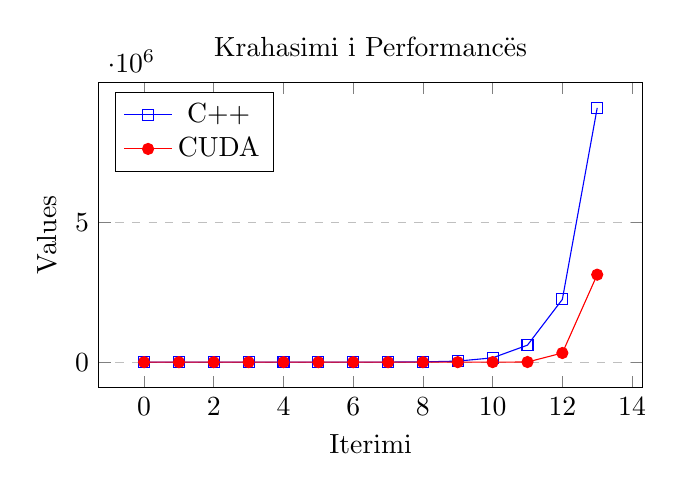
\begin{tikzpicture}
\begin{axis}[
    title={Krahasimi i Performancës},
    xlabel={Iterimi},
    ylabel={Values},
    legend pos=north west,
    ymajorgrids=true,
    grid style=dashed,
    width=0.7\textwidth,  % Adjusted width
    height=0.45\textwidth, % Adjusted height
]
\addplot[
    color=blue,
    mark=square,
    ]
    coordinates {
    (0,2)(1,3)(2,16)(3,17)(4,50)(5,140)(6,787)(7,2514)(8,9101)(9,37411)(10,154053)(11,607546)(12,2240534)(13,9075431)
    };
\addplot[
    color=red,
    mark=*,
    ]
    coordinates {
    (0,23)(1,26)(2,41)(3,29)(4,37)(5,25)(6,27)(7,60)(8,93)(9,409)(10,1384)(11,5032)(12,326359)(13,3123194)
    };
\legend{C++, CUDA}
\end{axis}
\end{tikzpicture}
\caption{Grafiku i krahasimit të performancës.}
\label{fig:koch_graph}
\end{figure}

\newpage

\begin{figure}[htp]
\centering
\subfigure[Koch Snowflake\label{fig:koch_snowflake_13}]{\includegraphics[width=0.8\linewidth]{koch_7.png}}
\subfigure[Koch Anti-Snowflake]{\label{fig:koch_anti}\includegraphics[width=0.8\linewidth]{koch_8.png}}
\caption{Fraktali në iterimin 11 i gjeneruar me CUDA.}
\label{fig:koch_big}
\end{figure}


% \begin{figure}[htp]
% \begin{figure}
%     \centering
%     \includegraphics[width=1\linewidth]{koch_8.png}
%     \caption{Enter Caption}
%     \label{fig:enter-label}
% \end{figure}
%     \centering
%     \includegraphics[width=0.6\linewidth]{koch_8.png}
%     \caption{Enter Caption}
%     \label{fig:enter-label}
% \end{figure}


\chapter{Fractal Tree}

\noindent Fractal Tree është një fraktal i njohur që përfaqëson vizualisht konceptin e rekursionit në natyrë. Ndërtimi i këtij fraktali fillon me një trung të vetëm, i cili më pas ndahet në dy degë në një kënd të caktuar. Secila prej këtyre degëve ndahet më tej në dy degë më të vogla, duke vazhduar këtë proces në mënyrë rekursive \cite{fractal_geometry}. Iterimet e para të këtij fraktali janë  paraqitur në figurën \ref{fig:tree_grow}. Me rritjen e iterimeve do të fitohet figura \ref{fig:tree_big}.

\begin{figure}[htbp!]
\centering
\subfigure[Iterimi 2]{\includegraphics[width=83px,height=90px]{tree_1}}
\subfigure[Iterimi 4]{\includegraphics[width=83px,height=90px]{tree_2}}
\subfigure[Iterimi 7]{\includegraphics[width=83px,height=90px]{tree_3}}
\subfigure[Iterimi 7]{\includegraphics[width=83px,height=90px]{tree_4}}
\caption{Rritja e pemës fraktale}
\label{fig:tree_grow}
\end{figure}

\section{Konstruktimi i degëve}

Le të jenë pikat \( A(x_1, y_1) \) dhe \( B(x_2, y_2) \). Duhet të gjejmë pikën \( C(c_1, c_2) \) ashtu që \( \overrightarrow{AB} = \lambda \overrightarrow{BC} \), dhe pikat \( C' \) dhe \( C'' \) ashtu që \( \angle CBC' = \alpha = \angle CBC'' \) (figura \ref{fig:fractal_construction}).


\begin{figure}[htpb]
    \centering
    \includegraphics[width=1\linewidth]{tree_5.png}
    \caption{Konstruktimi i degës.}
    \label{fig:fractal_construction}
\end{figure}



\noindent \\ Nga barazimi \( \overrightarrow{AB} = \lambda \overrightarrow{BC} \) marrim

\[
(x_2 - x_1, y_2 - y_1) = \lambda (c_1 - x_2, c_2 - y_2)
\]

\noindent \\ Duke barazuar kordinatat përkatëse të dysheve të renditura në të dy anët e barazimit marrim

\[
x_2 - x_1 = \lambda (c_1 - x_2)
\]
\[
y_2 - y_1 = \lambda (c_2 - y_2)
\]


\noindent \\Duke zgjidhur për \(c_1\), \(c_2\) fitojmë:

\[
c_1 = \frac{x_2 (1 + \lambda) - x_1}{\lambda}
\]

\[
c_2 = \frac{y_2 (1 + \lambda) - y_1}{\lambda}
\]

\noindent \\ Pikën \( C \) e rrotullojmë rreth pikës \( B \) për këndin \( \alpha \) dhe fitojmë pikën \( C'' \) me koordinatat:

\[
c_1'' = (c_1 - x_2) \cos(\alpha) - (c_2 - y_2) \sin(\alpha) + x_2
\]

\[
c_2'' = (c_1 - x_2) \sin(\alpha) + (c_2 - y_2) \cos(\alpha) + y_2
\]


\noindent \\ Ngjashëm, pika \( C' \) fitohet duke rrotulluar pikën \( C \) rreth pikës \( B \) për këndin \(-\alpha\).





\section{Numri i pikave të figurës}

\noindent \\ Le të jetë \( f(n) \) numri i brinjëve të figurës në iterimin \( n \). Pas secilit iterim, numri i brinjëve dyfishohet dhe kemi:

\[ f(n) = 2^0 + 2^1 + 2^2 + \cdots + 2^n = 2^{n+1} - 1. \]

\noindent \\ Secila brinjë ka dy pika dhe numri i pikave do të jetë \( 2 \cdot f(n) \), dhe këtë shprehje e përdorim për të lidhur pikat si segmente në pjesën e vizualizimit. \\

\begin{lstlisting}
void renderTreeFromBuffer() {
    glVertexAttribPointer(0, 2, GL_FLOAT, GL_FALSE, 0, nullptr);
    glEnableVertexAttribArray(0);
    glColor3f(0.0f, 0.0f, 0.0f);
    int numberOfVertices = 2 * (pow(2, iteration + 1) - 1);
    glDrawArrays(GL_LINES, 0, numberOfVertices2(iterations));
    glutSwapBuffers();	
}
\end{lstlisting}

\section{Paralelizimi}
\noindent Paralelizimi ndodh në menyrë hiearkike, ku në secilin iterim do të jenë aktiv një numër i caktuar i thredave. Secili thread aktiv do e marë degën  e \(i\) -të të figurës, dhe do e konstruktoj degën e djathtë ose të majtë varësisht nga indeksi. Dega e re e fituar futet në vargun e të gjitha degëve. Madhësia e këtij vargu do të jetë \( f(n) \).

\noindent \\ Për secilin iterim do të jenë \(2^n \) threada aktiv. Me rritje të iterimeve, numri i thredave aktiv do të  ngritet eksponencialisht: 

\begin{enumerate}
    \item Iterimi 0: Vetëm threadi me id 0 të jetë aktiv. Ky thread inicalizon degën fillestare.
    \item Iterimi 1: Threadat 2 dhe 3 janë aktiv. Threadi 2 konstrukton degën e majtë nga dega fillestare dhe e fut në vargun e degëve në pozitën 2. Threadi 3 do konstrukton degën e djathtë dhe e fut në vargun e degëve në pozitën 3.
    \item Iterimi 2: Threadat 4,5,6,7 janë aktiv. Thredat 3 dhe 4 konstruktojnë dëgën e majtë dhe të djathtë të degës nga pozita 2 e vargut.  Thredat 5,6 konsturktojnë degën e majtë dhe të djathtë, rrespektivisht, të degës nga pozita 3 e vargut. Deget e krijuara futen në vargun e degëve për iterimin e ardhshëm. 
    \item Iterimi \(n\): Threadat \(2^n\) deri në \(2^{n+1}-1\) do të jenë aktiv. Këta threada marin degët përkatëse, dhe varësisht nga indeksi konstruktojnë degë të djathtë ose të majtë.  
\end{enumerate}


\begin{figure}[htbp]
    \centering
    \includegraphics[width=1\linewidth]{tree_6.png}
    \caption{Ekzekutimi paralel i thredave.}
    \label{fig:tree_threads}
\end{figure}


\noindent \\ Paralelizimi dhe shtimi i të dhënave është modeluar në një graf binar (figura \ref{fig:tree_threads}). Çdo nyje në graf përfaqëson një thread që ndërton një degë, ndërsa degët e grafit përfaqësojnë ndarjen degës në iteracionet e ardhshme. Secili thread \(i\)  merr degën nga pozicioni prind \(i/2\) nga vargu i degëve, e konstrukton degën e djathtë ose të majtë, dhe dega e re e konstruktuar futet në pozicionin  \(i\)  të vargut. Secili nivel i grafit përfaqëson threadat të cilët janë duke punuar në paralel. 

\noindent \\ Indeksi më i majtë në nivelin \(n\) të grafit është:
\[ \text{leftMost}(n) = 2^n \]
\noindent Indeksi më i djathtë në nivelin \(n\) të grafit është:
\[ \text{rightMost}(n) = \text{leftMost}(n+1) - 1 = 2^{n+1} - 1 \]
\noindent  Numri i thredave që punojnë në paralel në nivelin \(n\) është:
\[ \text{leftMost}(n+1) - \text{leftMost}(n) = 2^{n+1} - 2^n = 2^n \]

\section{Kerneli}

\noindent Kerneli i mëposhtëm gjeneron fraktalin përmes llogaritjes paralele. Fillimisht threadi me indeks 0 trajton degën inicializuese. Për secilin iterim threads ndërmjet intervalit start\_at dhe end\_at janë aktiv dhe konstruktojnë degët e reja. Threads me indeks numër çift konstruktojnë degët e majta, kurse thredat me numër tek konstruktojnë degët e djathta.  Degët e konstruktuara ruhen në vargun e degëve të cilat do të ndahen në iterimin e ardshëm. Dy kulmet e degës i shtohen vargut points. Sinkronizimi siguron që të gjitha threadat përfundojnë detyrën e tyre para sa te të vazhdojnë në iterimin e ardhshëm. \\

\begin{lstlisting}
__global__ void branchDivide(float* points, Branch branch, Branch* branches, float angle_left, float angle_right, int start_iteration, int max_iterations, int threadShiftIndex) {

    int idx = threadIdx.x + blockIdx.x * blockDim.x;;
    idx += threadShiftIndex;
    
    Branch childBranch,parentBranch;
    float angle;
    auto g = cg::this_grid();
    
    if (idx == 0) {
        points[0] = branch.start.x;
        points[1] = branch.start.y;
        points[2] = branch.end.x;
        points[3] = branch.end.y;
        branches[1] = branch;
    }
    
    for (int iteration = start_iteration; iteration <= max_iterations; iteration++) {
        float start_at = round(pow(2, iteration));
        int end_at = round((pow(2, iteration + 1))) - 1;
    
        if (idx >= start_at && idx <= end_at) {
            int parentNode = idx / 2;
            parentBranch = branches[parentNode];
            int t = idx % 2;
            
            if (t == 0) {
                angle = angle_left;
            }
            else {
                angle = angle_right;
            }
            
            childBranch = makeChildBranch(parentBranch,angle);
            branches[idx] = childBranch;
            //add points to points array;
            int offset = 2 * 2 * (idx - 1);
            points[offset] = childBranch.start.x;
            points[offset + 1] = childBranch.start.y;
            points[offset + 2] = childBranch.end.x;
            points[offset + 3] = childBranch.end.y;
        }
    g.sync();
    }
}
\end{lstlisting}

\section{Krahasimet}

 Tabela \ref{tab:tree_table} krahason kohën e ekzekutimit në mikrosekonda të fraktalit ndërmjet versionit sekuencial dhe të versionit paralel. Implementimi me CUDA është bërë me  anë të grupeve kooperative, me 23040 threada për një thirrje të kernelit. Vizualizimi i këtyre rezultateve është në figurën \ref{fig:tree_graph}.
 
\begin{table}[h]
\centering
\resizebox{0.3\textwidth}{!}{%
\begin{tabular}{|l|l|l|}
\hline
Iterimi & C++ & CUDA \\ \hline
0 & 23 & 27 \\ \hline
1 & 40 & 25 \\ \hline
2 & 47 & 23 \\ \hline
3 & 39 & 28 \\ \hline
4 & 40 & 27 \\ \hline
5 & 58 & 27 \\ \hline
6 & 332 & 29 \\ \hline
7 & 288 & 28 \\ \hline
8 & 105 & 26 \\ \hline
9 & 155 & 26 \\ \hline
10 & 436 & 27 \\ \hline
11 & 541 & 24 \\ \hline
12 & 733 & 29 \\ \hline
13 & 1563 & 29 \\ \hline
14 & 2576 & 43 \\ \hline
15 & 4861 & 47 \\ \hline
16 & 9027 & 89 \\ \hline
17 & 22230 & 148 \\ \hline
18 & 37435 & 253 \\ \hline
19 & 75886 & 382 \\ \hline
20 & 145146 & 745 \\ \hline
21 & 294950 & 1268 \\ \hline
22 & 584644 & 2560 \\ \hline
23 & 1184101 & 5265 \\ \hline
24 & 2347734 & 142678 \\ \hline
25 & 4705941 & 439919 \\ \hline
26 & 9416423 & 789610 \\ \hline
\end{tabular}
}
\caption{Krahasimi i performancës.}
\label{tab:tree_table}
\end{table}

\begin{figure}[h]
\centering
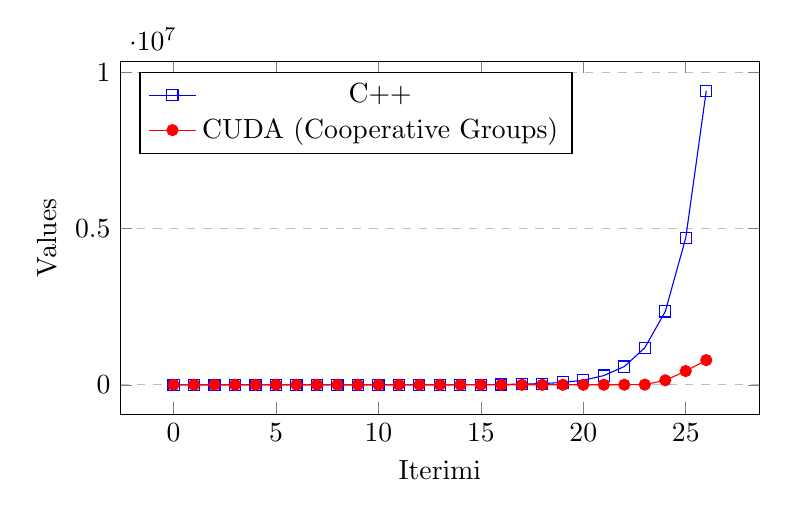
\begin{tikzpicture}
\begin{axis}[
    title={},
    xlabel={Iterimi},
    ylabel={Values},
    legend pos=north west,
    ymajorgrids=true,
    grid style=dashed,
    width=0.8\textwidth,  % Adjust width as needed
    height=0.5\textwidth, % Adjust height as needed
]
\addplot[
    color=blue,
    mark=square,
    ]
    coordinates {
    (0,23)(1,40)(2,47)(3,39)(4,40)(5,58)(6,332)(7,288)(8,105)(9,155)(10,436)(11,541)(12,733)(13,1563)(14,2576)(15,4861)(16,9027)(17,22230)(18,37435)(19,75886)(20,145146)(21,294950)(22,584644)(23,1184101)(24,2347734)(25,4705941)(26,9416423)
    };
\addplot[
    color=red,
    mark=*,
    ]
    coordinates {
    (0,27)(1,25)(2,23)(3,28)(4,27)(5,27)(6,29)(7,28)(8,26)(9,26)(10,27)(11,24)(12,29)(13,29)(14,43)(15,47)(16,89)(17,148)(18,253)(19,382)(20,745)(21,1268)(22,2560)(23,5265)(24,142678)(25,439919)(26,789610)
    };
\legend{C++, CUDA (Cooperative Groups)}
\end{axis}
\end{tikzpicture}
\caption{Grafiku i krahasimit të performancës.}
\label{fig:tree_graph}
\end{figure}



\newpage


% \begin{figure}
%     \centering
%     \includegraphics[width=0.90\linewidth]{tree_7.png}
%     \caption{Enter Caption}
%     \label{fig:enter-label}
% \end{figure}


\begin{figure}[]
    \centering
    \makebox[\textwidth]{\includegraphics[width=1.7\linewidth]{tree_7.png}}
    \caption{Pema fraktale në iterimin 24 e gjeneruar me CUDA.}
    \label{fig:tree_big}
\end{figure}

\chapter{Sierpinski Triangle}

\noindent \\ Trekëndëshi i Sierpinskit është një fraktal i famshëm i emëruar pas matematikanit Waclaw Sierpinski. Fraktali mund të konstruktohet duke filluar nga një trekëndësh barabrinjësh dhe pastaj rekursivisht duke ndarë çdo trekëndësh si vijon:

\begin{enumerate}
    \item Në secilën brinjë të trekëndëshit gjejë pikën e mesit dhe bashkoj këto pika, ku formohen katër trekëndësha të rinjë.
    \item Përsërit procesin në secilin trekëndësh përveç trekëndëshit të mesëm.
\end{enumerate}

\noindent Katër iterimet e para të fraktalit janë paraqitur në figurën \ref{fig:sierpinski_iterations}. Me rritjen e iterimeve do të fitohet figura \ref{fig:sierpinski_big}.

\begin{figure}[htbp]
\hfill
\subfigure[Iterimi 0]{\includegraphics[width=0.24\linewidth]{triangle_1}}
\hfill
\subfigure[Iterimi 1]{\includegraphics[width=0.24\linewidth]{triangle_2}}
\hfill
\subfigure[Iterimi 2]{\includegraphics[width=0.24\linewidth]{triangle_3}}
\hfill
\subfigure[Iterimi 3]{\includegraphics[width=0.24\linewidth]{triangle_4}}
\hfill
\caption{Iterimet e para të fraktalit.}
\label{fig:sierpinski_iterations}
\end{figure}


\section{Konstruktimi i trekëndëshit të mbrendshëm}

Le të jetë dhënë trekëndëshi \( \triangle ABC \) dhe pikat \( D, E, F \) që përgjysmojnë brinjët e trekëndëshit (figura \ref{fig:triangle_construction}). Kordinatat e pikave \( D, E, F \) janë:


\[ D = \left( \frac{a_1 + b_1}{2}, \frac{a_2 + b_2}{2} \right) \]
\[ E = \left( \frac{b_1 + c_1}{2}, \frac{b_2 + c_2}{2} \right) \]
\[ F = \left( \frac{a_1 + c_1}{2}, \frac{a_2 + c_2}{2} \right) \]

\noindent \\ Trekëndëshat \( \triangle ADF \), \( \triangle DBE \), \( \triangle FEC \), do të hyjnë në iterimin e ardhshëm për ndarje.

\begin{figure}
    \centering
    \includegraphics[width=0.55\linewidth]{triangle_5.png}
    \caption{Konstruktimi i trekëndëshit të mbrendshëm.}
    \label{fig:triangle_construction}
\end{figure}

\section{Numri i pikave të figurës}

Në vizualizim të fraktalit, do të renderohet trekëndëshi fillestar me ngjyrë të gjelbërt dhe trekëndëshat e mbrendshëm me ngjyrë të zezë. Nevoitet të gjendet numri i pikave të trekëndëshave të mbrendshëm (të zi). Shënojmë me \( T(n) \) numrin e trekëndëshave që shtohen nga iterimi \( n-1 \) në \( n \). Pra në \( T(1) = 1 \), \( T(2) = 3 \), \( T(3) = 9 \). Secili trekëndësh pas ndarjes jep 3 trekëndësha të rinj në të cilët do konstruhohen trekëndëshat e zi.

\[ 
T(n) = 3T(n-1) = 3^2 T(n-2) = \cdots = 3^{n-1} T(1) = 3^{n-1} 
\]

\noindent \\ Numri i të gjithë trekëndëshave të zi në iterimin \(n\)  është shuma:
\[
T(1) + T(2) + \cdots + T(n) = 3^0 + 3^1 + \cdots + 3^{n-1} = \sum_{i=0}^{n-1} 3^i = \frac{3^n - 1}{2}
\]
\noindent Secili trekëndësh ka tre pika, dhe nëse llogarisim edhe 3 pikat e trekëndëshit fillestar kemi

\[
f(n) = 3 + \frac{3 \cdot (3^n - 1)}{2} = 3 + \frac{3^{n+1} - 3}{2} = \frac{3}{2} (3^n + 1)
\]

\noindent  Vargu \(f(n)\) paraqet numrin e të gjithë pikave të trekëndshave të brendshëm dhe të trekëndëshit fillestar në iterimin \(n\). Fillimisht kemi vizualisuar trekëndëshin inicializues me ngjyrë të gjelbërt (rreshti 6), dhe pastaj trekëndëshat e zi në rreshtin 10. \\ 

\begin{lstlisting}
void renderTriangleFromBuffer() {
 glVertexAttribPointer(0, 2, GL_FLOAT, GL_FALSE, 0, nullptr);
 glEnableVertexAttribArray(0);
 //Render first green triangle
 glColor3f(0.29f, 0.44f, 0.55f);
 glDrawArrays(GL_TRIANGLES, 0, 3);
 //Render blackTriangles
 int numberVerticesBlackTriangles = (pow(3, iterations + 1) - 3) / 2;
 glColor3f(0.0f, 0.0f, 0.0f);
 glDrawArrays(GL_TRIANGLES, 3, numberVerticesBlackTriangles);
 glutSwapBuffers();
} 
\end{lstlisting}


\section{Paralelizimi}

Paralelizimi ndodh në menyrë hiearkike, ku në secilin iterim do të jenë aktiv një numër i caktuar i thredave. Secili thread aktiv do e marë trekëndëshin e \(i\) -të të figurës, dhe do i gjejë tre pikat për ndërtimin e trekëndëshit të mbrendshëm. Tre trekëndëshat që do të ndahen në iterimin e ardshëm, definohen nga secili thread dhe futen në vargun e të gjithë trekëndëshave. Madhësia e këtij vargu do të jetë numri i pikave të trekëndëshave të gjetur në formulën në raport me 3, sepse secili trekëndësh ka tri pika.

\[
\frac{f(n)}{3} = \frac{1}{2} (3^n + 1)
\]



\noindent \\ Për secilin iterim do të jenë \(3^n\) threada aktiv. Me rritje të iterimeve, numri i thredave aktiv do të ngirtet eksponencialisht:
\begin{itemize}
    \item Iterimi 0: Vetëm threadi me id 0 të jetë aktiv. Ky thread inicalizon trekëndëshin fillestar.
    \item Iterimi 1: Vetëm threadi me id 1 është aktiv. Ky thread ndërton trekëndëshin e parë të mbrendshëm. Tre trekëndëshat definohen dhe futen në vargun e trekëndëshave në pozitat 2,3,4, të cilët do ndahen në iterimin e ardhshëm.
    \item Iterimi  2: Threadat 2,3,4 janë aktiv. Secili thread mer trekëndëshin përkatës në bazë të indeksit të tyre. Secili thread ndërton trekëndëshin e mbrendshëm, definon 3 trekëndëshat, të cilët futen në vargun e të gjithë trekëndëshave.
    \item Iterimi \(n\): Threadat \(\frac{3^n + 1}{2}\) deri në \(\frac{3^{n+1} - 1}{2}\) do të jenë aktiv. Këta threada marrin trekëndëshat nga iterimi i kaluar dhe ndërtojnë trekëndëshat e mbrendshëm në ta.
\end{itemize}

\begin{figure}[]
    \centering
    \includegraphics[width=0.3\linewidth]{triangle_6.png}
    \caption{Nyja me fëmijë në graf ternar.}
    \label{fig:node_ternary}
\end{figure}

\begin{figure}[htpb]
    \centering
    \includegraphics[width=1\linewidth]{triangle_7.png}
    \caption{Sinkronizimi dhe ekzekutimi paralel.}
    \label{fig:sierpinski_parallel}
\end{figure}

\noindent \\ Paralelizimi dhe shtimi i të dhënave është modeluar në një graf ternar si në figurën \ref{fig:sierpinski_parallel}. Çdo nyje në graf ternar përfaqëson një thread që ndërton trekëndëshat e mbrendshëm, ndërsa degët përfaqësojnë ndarjen e tre trekëndëshave në iteracionet e ardhshme. Secili thread \(i\)  merr trekëndëshin \(i\) nga vargu i trekëndëshave, e ndan atë, dhe shton tre trekëndësha të ri në pozitat  fëmijë \(3i-1,3i,3i+1\) (figura \ref{fig:node_ternary}). Secili nivel i grafit përfaqëson threadat të cilët janë duke punuar në paralel. 

\noindent \\ Indeksi më i djathtë i nivelit \(n\) të grafit është pikërisht shuma:
\[
\text{rightMost}(n) = \sum_{i=0}^n 3^i = \frac{3^{n+1} - 1}{2}
\]
\noindent Indeksi më i majtë i nivelit \(n\) të grafit është:
\[
\text{leftMost}(n) = \text{rightMost}(n-1) + 1 = \frac{3^n - 1}{2} + 1 = \frac{3^n + 1}{2}
\]
\noindent Numri i thredave që punojnë në paralel në nivelin \(n\):
\[
\text{leftMost}(n+1) - \text{leftMost}(n) = \frac{3^{n+1} + 1}{2} - \frac{3^n + 1}{2} = 3^n
\]

\section{Kerneli}

Kerneli i mëposhtëm gjeneron fraktalin përmes llogaritjes paralele. Fillimisht threadi me indeks 0 trajton trekëndëshin inicializues. Për secilin iterim threads ndërmjet intervalit start\_at dhe end\_at janë aktiv dhe llogaritin meset e segmenteve të trekëndëshit. Definohen tri trekëndësha të rinjë të cilët ruhen në vargun e trekëndshëva që do të ndahen. Meset e segmenteve i shtohen vargut points për vizualizim të trekëndëshit. Sinkronizimi siguron që të gjitha threadat përfundojnë detyrën e tyre para sa te të vazhdojnë në iterimin e ardhshëm.  \\

\begin{lstlisting}
__global__ void kernel(float* points, Triangle* triangles, int start_iteration, int max_iteration, int threadShiftIndex) {
    int idx = threadIdx.x + blockDim.x * blockIdx.x;
    idx += threadShiftIndex;
    Point A,B,C,A1,B1,C1;
    Triangle triangle,t_1,t_2t_3;
    auto g = cg::this_grid();
    if (idx == 0) {
    triangles[1] = triangle;
    }
    
    for (int iteration = start_iteration; iteration <= max_iteration; iteration++) {
        int start_at = (round((pow(3, iteration) + 1))) / 2;
        int end_at = (round((pow(3, iteration+1) - 1))) / 2;
        if (idx >= start_at && idx <= end_at) {
            triangle = triangles[idx];
            A = triangle.A;
            B = triangle.B;
            C = triangle.C;
            //DivideTriangle 
            A1.x = (A.x + B.x) / 2.0f;
            A1.y = (A.y + B.y) / 2.0f;
            B1.x = (B.x + C.x) / 2.0f;
            B1.y = (B.y + C.y) / 2.0f;
            C1.x = (C.x + A.x) / 2.0f;
            C1.y = (C.y + A.y) / 2.0f;
            //Make three new Triangles
            t_1.A = A;
            t_1.B = A1;
            t_1.C = C1;
            
            t_2.A = A1;
            t_2.B = B;
            t_2.C = B1;
            
            t_3.A = C1;
            t_3.B = B1;
            t_3.C = C;
            //Insert three new triangles to triangles array
            triangles[3 * idx - 1] = t_1;
            triangles[3 * idx] = t_2;
            triangles[3 * idx + 1] = t_3;
            
            //Add three points 
            int offset = 2 * 3 * (idx);
            points[offset] = A1.x;
            points[offset + 1] = A1.y;
            points[offset + 2] = B1.x;
            points[offset + 3] = B1.y;
            points[offset + 4] = C1.x;
            points[offset + 5] = C1.y;
        }
        g.sync();
    }
}

\end{lstlisting}


\section{Krahasimet}

Tabela \ref{tab:sierpinski_table} krahason kohën e ekzekutimit në mikrosekonda të fraktalit ndërmjet versionit sekuencial dhe të versionit paralel. Implementimi me CUDA është bërë me  anë të grupeve kooperative, me 25600 threada për një thirrje të kernelit. Vizualizimi i këtyre rezultave është në figurën \ref{fig:sierpinski_graph}.

\begin{table}[h]
\centering
\resizebox{0.4\textwidth}{!}{%
\begin{tabular}{|l|l|l|}
\hline
Iterimi & C++ & CUDA( \\ \hline
0 & 1 & 32 \\ \hline
1 & 2 & 23 \\ \hline
2 & 3 & 23 \\ \hline
3 & 3 & 31 \\ \hline
4 & 5 & 20 \\ \hline
5 & 19 & 23 \\ \hline
6 & 47 & 19 \\ \hline
7 & 133 & 23 \\ \hline
8 & 257 & 22 \\ \hline
9 & 861 & 37 \\ \hline
10 & 2633 & 34 \\ \hline
11 & 8374 & 82 \\ \hline
12 & 30457 & 243 \\ \hline
13 & 74373 & 653 \\ \hline
14 & 271835 & 1886 \\ \hline
15 & 1060085 & 6367 \\ \hline
16 & 5812052 & 2782181 \\ \hline
17 & 14557977 & 6679207 \\ \hline
\end{tabular}
}
\caption{Krahasimi i performancës.}
\label{tab:sierpinski_table}
\end{table}



\begin{figure}[h]
\centering
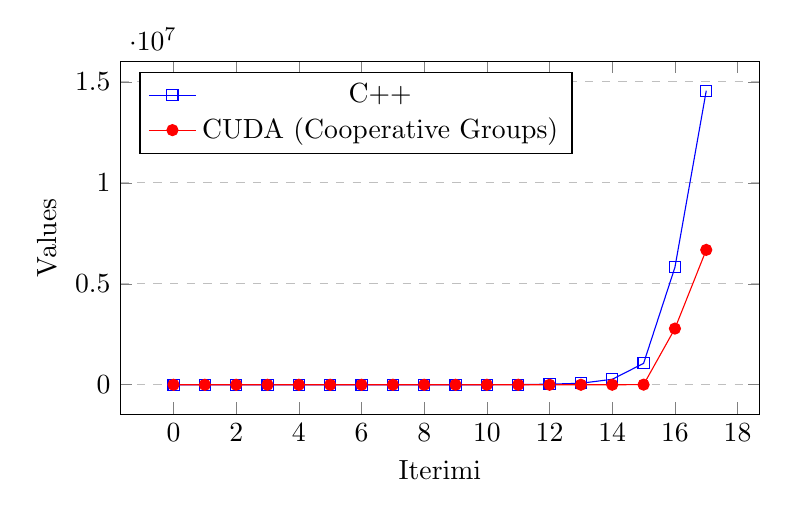
\begin{tikzpicture}
\begin{axis}[
    title={},
    xlabel={Iterimi},
    ylabel={Values},
    legend pos=north west,
    ymajorgrids=true,
    grid style=dashed,
    width=0.8\textwidth,  % Adjust width as needed
    height=0.5\textwidth, % Adjust height as needed
]
\addplot[
    color=blue,
    mark=square,
    ]
    coordinates {
    (0,1)(1,2)(2,3)(3,3)(4,5)(5,19)(6,47)(7,133)(8,257)(9,861)(10,2633)(11,8374)(12,30457)(13,74373)(14,271835)(15,1060085)(16,5812052)(17,14557977)
    };
\addplot[
    color=red,
    mark=*,
    ]
    coordinates {
    (0,32)(1,23)(2,23)(3,31)(4,20)(5,23)(6,19)(7,23)(8,22)(9,37)(10,34)(11,82)(12,243)(13,653)(14,1886)(15,6367)(16,2782181)(17,6679207)
    };
\legend{C++, CUDA (Cooperative Groups)}
\end{axis}
\end{tikzpicture}
\caption{Grafiku i krahasimit të performancës.}
\label{fig:sierpinski_graph}
\end{figure}


\newpage


\begin{figure}[]
    \centering
    \makebox[\textwidth]{\includegraphics[width=1.8\linewidth]{triangle_8.png}}
    \caption{Trekëndëshi i Sierpinskit në iterimin 7 i gjeneruar me CUDA.}
    \label{fig:sierpinski_big}
\end{figure}


\chapter{Mandelbrot Set}

\noindent Mandelbrot Set, është një fraktal i emërtuar pas Benoit B. Mandelbrot, definuar sipas funksionit rekursiv \( z_{n+1} = z_n^2 + c \), ku \( z \) dhe \( c \) janë numra kompleks. Duke filluar me \( z_0 = 0 \), numri kompleks \( c \) i takon Mandelbrot set nëse vargu \( z_n \) është i kufizuar kur \( n \to \infty \). Për shembull, pika \( c = 1 \) nuk është element i bashkësisë Mandelbrot sepse për \( c = 1 \), vargu \( 0, 1, 2, 5, 26 \) tenton në pafundësi. Pika \( c = -1 \) është element i bashkësisë Mandelbrot sepse vargu \( 0, -1, 0, -1, 0, \ldots \) është i kufizuar. Teorema 1 do të na ndihmoj në vizualizimin e fraktalit \cite{complex_analysis}.

\noindent \\ \textbf{Teorema 1.} Numri kompleks \( c \) i takon bashkësisë Mandelbrot atëherë dhe vetëm atëherë kur \( |z_n| \leq 2 \) për çdo \( n \geq 1 \).

\noindent \\Secili piksell i imazhit reprezenton një pikë në sistemin koordinativ dhe për atë pikë e testojme nëse \( |z_n| \leq 2 \) pas \(n_\text{max}\) iterimeve. Nëse me ngjyrë te zezë ngjyrosim pikat që i takojne bashkësisë dhe me ngjyrë të bardhë pikat që nuk i takojnë bashkësisë, atëherë do të fitojmë imazhin në figurën \ref{fig:mandelbrot_bw}.

\begin{figure}[h]
    \centering
    \includegraphics[width=0.4\linewidth]{mandelbrot_1.png}
    \caption{Mandelbrot Set bardhë dhe e zëzë.}
    \label{fig:mandelbrot_bw}
\end{figure}

\section{Pasqyrimi i piksellëve në sistemin kordinativ}
Për pasqyrim të pikselëve në sistem koordinativ, e përdorim ekuacionin e drejtëzës. Le të jetë 
imazhi \(I\) me dimensione \(w \times h\). Le të jenë pikat \((x_1, y_2)\) dhe \((x_2, y_2)\), pikat e fillimit dhe mbarimit 
të sistemit koordinativ në të cilin imazhi duhet të pasqyrohet si në figurën \ref{fig:image_coordinate}. Secili piksell \((i, j)\) duhet të 
reprezentojë një pikë \((x, y)\) në sistemin koordinativ. Për shembull, pikselli \((0, 0)\) pasqyrohet në \((x_1, y_2)\).


\noindent \\ Intervali $[0,w]$ duhet të pasqyrohet në $[x_1,x_2]$ dhe intervali $[0,h]$ duhet të pasqyrohet në $[y_1,y_2]$. Definojmë pasqyrimet $f_r$, $f_y$ për këto intervale.

\[
f_r : [0, w] \rightarrow [x_1, x_2]
\]
\[
f_c : [0, h] \rightarrow [y_1, y_2]
\]

\noindent \\Për kordinatat \(x\) vlenë
\[
f_r(0) = x_1
\]
\[
f_r(w) = x_2
\]

\noindent Transformimi linear për kordinatat $x$ mund të fitohet si ekuacioni i drejtëzës së pikave $(0, x_1)$ dhe $(w, x_2)$.

\[
\frac{i - 0}{w - 0} = \frac{x - x_1}{x_2 - x_1}
\]

\begin{figure}[h]
    \centering
    \includegraphics[width=0.6\linewidth]{image_to_coordinate.png}
    \caption{Piksellët në sistem kordinativ.}
    \label{fig:image_coordinate}
\end{figure}

\noindent \\ Duke zgjidhur për $x$ fitojmë
\[
\frac{i - 0}{w - 0} = \frac{x - x_1}{x_2 - x_1} \implies \frac{i}{w} = \frac{x - x_1}{x_2 - x_1} \implies x - x_1 = \frac{i}{w} (x_2 - x_1) \implies x = \frac{i}{w} (x_2 - x_1) + x_1
\]

\noindent \\ Në mënyrë krejtësisht analoge fitojmë

\[
y = \frac{j}{w} (y_2 - y_1) + y_1
\]

\noindent \\ Përfundimisht, pikselli $(i,j)$ pasqyrohet në pikën $(x,y)$ në sistemin kordinativ me anë të këtyre formulave:
\[
x = \frac{i}{w} (x_2 - x_1) + x_1
\]
\[
y = \frac{j}{h} (y_2 - y_1) + y_1
\]

\section{Ngjyrosja e Mandelbrot}

\noindent \\ Ngjyrosja e bashkësisë të Mandelbrot ka të bëjë me caktimin e ngjyrave të pikave në rrafshin kompleks bazuar se sa shpejtë vargu \(z_n\) tenton në infinit. Do të na duhej një numër \(t\) prej 0 në 1 për të reprezentuar këtë shpejtesi. Kjo vlerë pastaj konvertohet në sistemin e ngjyrave HSV e pastaj në RGB. 

\noindent \\ Ka shumë mënyra se si mund të llogaritet numri \(t\). Le të jetë \(n_\text{max}\) numri maksimal i iterimeve. Le të jetë  \(n\) numri i iterimit në të cilin \(z_n\) ose shpëton nga bashkësia e Mandelbrot  (\(n< n_\text{max}\)) ose mbetet mrenda bashkësisë dhe nuk shpëton (\(n=n_\text{max}\)). Mënyra më bazike e llogaritjes së numrit \(t\) është:

\[ t = \frac{n}{n_{\text{max}}} \]

\noindent Një menyre tjetër është duke shfrytëzuar formulën që njihet si normalized iteration count \cite{complex_colors}. Formula ipet:  
\[  s = n + 1 - \frac{\log(\log(|z_n|))}{\log(2)}\]

\noindent Vlera \(s\) normalizohet ndaj numrit maksimal të iterimeve: 
\[t = \frac{s}{n_{\text{max}}}\]
% \begin{align*}
%    \\
    
% \end{align*}

\noindent \\ Le të jetë treshja e ngjyrave në sistemin HSV $(H_{HSV}, S_{HSV}, V_{HSV})$, ku $H_{HSV}, S_{HSV}$, dhe $V_{HSV} \in [0,1]$. Vlera e nuancës në rastin tonë do të jetë $H = t$, e ngopjes $S_{HSV} = 1$, dhe e ndriçimit $V_{HSV} = 1$. Konvertimi i kësaj treshe në sistemin RGB bëhet sipas procesit të mëposhtëm \cite{hsv_rgb}.

\begin{align*}
H' &= (6 \cdot H_{HSV}) \mod 6  \\
c_1 &= \lfloor H' \rfloor, \quad c_2 = H' - c_1 \\
x &= (1 - S_{HSV}) \cdot v \\
y &= (1 - (S_{HSV} \cdot c_2)) \cdot V_{HSV} \\
z &= (1 - (S_{HSV} \cdot (1 - c_2))) \cdot V_{HSV}
\end{align*}

\noindent  Bazuar në  vlerën e  $c_1$, vlerat e normalizuara $R', G', B' \in [0,1]$ llogariten nga $v = V_{HSV}$, $x$, $y$, dhe $z$ si vijon:

\[
(R', G', B') = 
\begin{cases}
    (v, z, x) & \text{nëse } c_1 = 0 \\
    (y, v, x) & \text{nëse } c_1 = 1 \\
    (x, v, z) & \text{nëse } c_1 = 2 \\
    (x, y, v) & \text{nëse } c_1 = 3 \\
    (z, x, v) & \text{nëse } c_1 = 4 \\
    (v, x, y) & \text{nëse } c_1 = 5.
\end{cases} 
\]

\noindent \\  Përfundimisht bëhet shkallëzimi i RGB në numra të plotë në intervalin $[0, N - 1]$ (zakonisht $N = 256$).

\[
R = \min(\text{round}(N \cdot R'), N - 1),
\]
\[
G = \min(\text{round}(N \cdot G'), N - 1),
\]
\[
B = \min(\text{round}(N \cdot B'), N - 1). 
\]

\noindent Aplikimi i këtyre ngjyrave rezulton në imazhin \ref{fig:big_mandelbrot} dhe pasi që zmadhojmë në fraktal ngjyrat duken si në figurën \ref{mandelbrot_minis}.

 \begin{figure}[htbp]
\centering
\subfigure[]{\includegraphics[width=83px,height=83px]{mandelbrot_3}}
\subfigure[]{\includegraphics[width=83px,height=83px]{mandelbrot_4}}
\subfigure[]{\includegraphics[width=83px,height=83px]{mandelbrot_5}}
\subfigure[]{\includegraphics[width=83px,height=83px]{mandelbrot_6}}
\caption{Zmadhimet në bashkësinë Mandelbrot.}
\label{mandelbrot_minis}
\end{figure}


\newpage
\section{Kerneli}
Kerneli i mëposhtëm gjeneron një imazh të bashkësisë Mandelbrot. Secili thread i korrespondon një piksell të këtij imazhi. Fillimisht llogariten kordinatat komplekse të secilit piksell bazuar në indeksin e thredave. Pastaj fillon iterimi duke përdorur formulën e Mandelbrot për të caktuar nëse një piksell shpëton nga bashkësia mbrenda një numër të caktuar të iterimeve. Ngjyrat RGB caktohen bazuar në numrin e iterimit në të cilën \(z_n\) terminohet, dhe ngjyrat ruhen në vargun dalës për vizualizim. \\

\begin{lstlisting}
   __global__ void kernel(uchar4* ptr, double zoomfactor, double shiftX, double shiftY, int iterations, int width, int height) {

    int i = threadIdx.x + blockIdx.x * blockDim.x;
    int j = threadIdx.y + blockIdx.y * blockDim.y;
        
    int offset = i + j * blockDim.x * gridDim.x;
        
    double aspectRatio = (1.0 * width) / (1.0 * height);
    double startIntervalX = (-2) * zoomfactor * aspectRatio;
    double endIntervalX = 1 * zoomfactor * aspectRatio;
    double startIntervalY = 1.5 * zoomfactor;
    double endIntervalY = -1.5 * zoomfactor;
        
    //Each pixel represents a point in the Oxy coordinate system. These points are 
    double x = (endIntervalX - startIntervalX) * i / (width * 1.0) + startIntervalX + shiftX;
    double y = (endIntervalY - startIntervalY) * j / (height * 1.0) + startIntervalY + shiftY;
        
    double c_x = x;
    double c_y = y;
    double zX = 0, zY = 0, a = 0, b = 0;
    int max_iteration = iterations;
    int iteration;
    double squaredSums;
    for (iteration = 0; iteration < max_iteration; iteration++) {
        double zX_squared = zX * zX;
        double zY_squared = zY * zY;
        a = zX_squared - zY_squared + c_x;
        b = 2 * zX * zY + c_y;
        zX = a;
        zY = b;
        squaredSums = zX_squared + zY_squared;
        if (squaredSums > 4) {
            break;
        }
    }
    int R = 0, G = 0, B = 0;
    if (iteration < max_iteration) {
    setRGB(squaredSums, iteration, max_iteration, R, G, B);
    }
    ptr[offset].x = R;
    ptr[offset].y = G;
    ptr[offset].z = B;
    ptr[offset].w = 0;
} 
\end{lstlisting}

\section{Krahasimet}

\noindent Tabela \ref{tab:mandelbrot_table} krahason kohën e ekzekutimit në mikrosekonda për iterime të ndryshme të fraktalit ndërmjet versionit sekuencial dhe të versionit paralel në rezolucion 1920x1080.  Vizualizimi i këtyre rezultateve është bërë në figurën \ref{fig:mandelbrot_graph}.

\vspace{10pt} % Add some vertical space before the table

\begin{table}[h]
\centering
\resizebox{0.45\textwidth}{!}{%
\begin{tabular}{|l|l|l|}
\hline
Iterime & Sekuencial & CUDA \\ \hline
100 & 733630 & 9400 \\ \hline
130 & 843132 & 10436 \\ \hline
160 & 937728 & 11135 \\ \hline
190 & 1072441 & 11930 \\ \hline
210 & 1133325 & 12447 \\ \hline
255 & 1266945 & 15498 \\ \hline
445 & 1935680 & 14152 \\ \hline
610 & 2493841 & 16123 \\ \hline
775 & 3098080 & 19263 \\ \hline
1065 & 4057208 & 30757 \\ \hline
2300 & 8331929 & 63800 \\ \hline
\end{tabular}
}
\caption{Krahasimi i performancës.}
\label{tab:mandelbrot_table}
\end{table}


\begin{figure}[h]
\centering
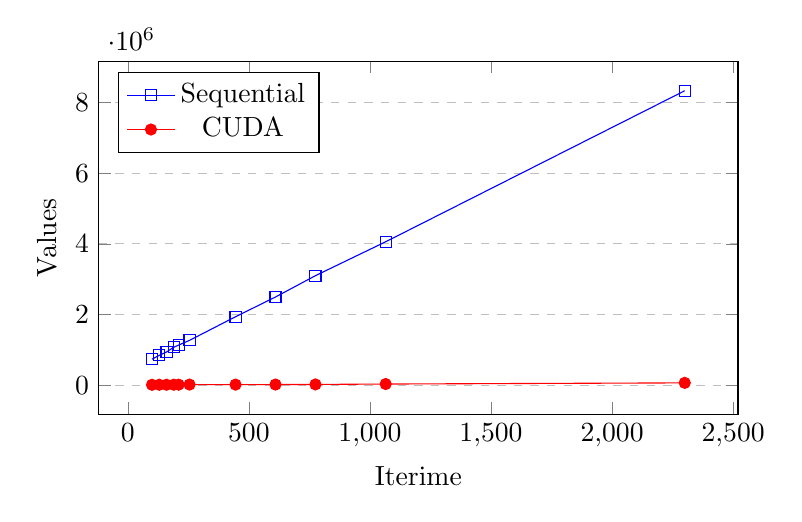
\begin{tikzpicture}
\begin{axis}[
    title={},
    xlabel={Iterime},
    ylabel={Values},
    legend pos=north west,
    ymajorgrids=true,
    grid style=dashed,
    width=0.8\textwidth,  % Adjust width as needed
    height=0.5\textwidth, % Adjust height as needed
]
\addplot[
    color=blue,
    mark=square,
    ]
    coordinates {
    (100,733630)(130,843132)(160,937728)(190,1072441)(210,1133325)(255,1266945)(445,1935680)(610,2493841)(775,3098080)(1065,4057208)(2300,8331929)
    };
\addplot[
    color=red,
    mark=*,
    ]
    coordinates {
    (100,9400)(130,10436)(160,11135)(190,11930)(210,12447)(255,15498)(445,14152)(610,16123)(775,19263)(1065,30757)(2300,63800)
    };
\legend{Sequential, CUDA}
\end{axis}
\end{tikzpicture}
\caption{Grafiku i krahasimit të performancës.}
\label{fig:mandelbrot_graph}
\end{figure}



\newpage

\begin{figure}[]
    \centering
    \makebox[\textwidth]{\includegraphics[width=1.6\linewidth]{mandelbrot_2}}
    \caption{Mandelbrot Set i gjeneruar me CUDA.}
    \label{fig:big_mandelbrot}
\end{figure}



\chapter{Përfundim}

Ky punim ka shtjelluar implementimin e programimit paralel për gjenerimin e fraktaleve dhe krahasimet në performancë ndaj versionit sekuencial. Duke përdorur CUDA, kemi arritur përmirësime të dukshme të performancës ndaj metodave tradicionale sekuenciale.  Implementimet në CUDA kanë reduktuar kohën e ekzekutimit dukshëm, veçanërisht në iteracione të larta. Këto rezultate dëshmojnë efektivitetin e llogaritjes paralele për trajtimin e punëve komplekse dhe intesive.
\begin{thebibliography}{9}

\bibitem{cuda_by_example}
Sanders, J., \& Kandrot, E. (2010). \emph{CUDA by example: an introduction to general-purpose GPU programming.} Addison-Wesley Professional.

\bibitem{cuda_guide}
NVIDIA Corporation (2024). \emph{CUDA C++ Programming Guide, Release 12.5}. NVIDIA Corporation.


\bibitem{opengl}
de Vries, J. (2020). \emph{Learn OpenGL: Learn Modern OpenGL Graphics Programming in a Step-by-step Fashion}. Kendall \& Welling.

\bibitem{fractal_geometry}
Mandelbrot, B. (1982). \emph{The Fractal Geometry of Nature}. Times Books.

\bibitem{complex_analysis}
Gamelin, T. W. (2013). \emph{Complex Analysis}. Springer.

\bibitem{complex_colors}
Garcia, F., Fernandez, A., Barrallo, J., Martin, L. (2002). \emph{Coloring Dynamical Systems in the Complex Plane}. The University of the Basque Country, Plaza de Oñati, 2, 20009 San Sebastián, Spain.

\bibitem{hsv_rgb}
Burger, W., Burge, M. J. (2007). \emph{Digital Image Processing: An Algorithmic Introduction using Java}, First Edition. Publisher.


\end{thebibliography}


\appendix
\chapter{Github repository}

https://github.com/drilonaliu/Bachelor-Thesis
\newpage
\end{document}